\section{Aplicación de ejemplo}

Para comprender mejor esta problemática veamos un ejemplo. Supongamos una simple
aplicación, donde los clientes de un banco pueden transferir dinero de
una cuenta a otra. Al realizar una transferencia, hay que extraer el monto
indicado de una cuenta, y depositarlo en otra. 
Al ejecutar cualquiera de estas dos operaciones se pueden producir errores,
como por ejemplo, que no haya saldo saldo suficiente, o que el depósito supere
el máximo permitido.

La figura \ref{example} muestra el diagrama de clases de la aplicación de
ejemplo

	\medskip

	\begin{figure}[h]
		\centering
		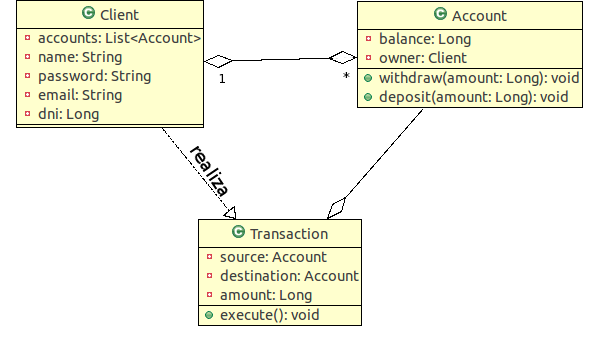
\includegraphics[width=250px, height=150px]{img/transaccion}
		\caption{Diagrama UML de la aplicación de ejemplo}
		\label{example}
	\end{figure}	
	
La aplicación de ejemplo tiene los siguientes casos de uso:

\begin{enumerate}
  \item{\bf{Transferir Dinero}} 
	Tres ventajas:
	- queda más simple
	- menos posibilidad de mandármela
	- concurrencia.
  	
  \item{\bf{Transferencias múltiples}}
	muchas transferencias en una única transacción\ldots fijate si sale algo y si no
	lo volamos.
\end{enumerate}

La figura \ref{executeTransaction} muestra el método  \lstinline|execute| de la
clase \lstinline|Transaction| \begin{figure}[h]
	\begin{lstlisting}
		public void execute(){
			this.source.withdraw(this.amount);
			this.destination.deposit(this.amount);
		}
	\end{lstlisting}
	\caption{Fragmento de código de la Clase Transaction}
	\label{executeTransaction}
\end{figure}
